\documentclass{article}
\usepackage[utf8]{inputenc}
\usepackage[english]{babel}
\usepackage{graphicx}
\usepackage{float}
\usepackage{listings}
\usepackage{hyperref}
\usepackage{amsmath}
\hypersetup{
    colorlinks=true,
    linkcolor=blue,
    filecolor=magenta,      
    urlcolor=cyan,
}
\urlstyle{same}

\title{Manual 4 - 2do Torneo de Programación Competitiva}
\author{Lions R.C.}
\date{Julio 2019}

\begin{document}

\maketitle

\tableofcontents

\begin{figure}[H]
    \centering
    
\includegraphics[width=0.2\paperwidth]{newblack}
\end{figure}

\section{Arreglos multidimensionales}

A veces es conveniente manejar datos como si fueran a estar en una matriz de más de una dimensión, asi que C++ te permite crear arreglos multidimensionales para facilitar este proceso. Casi nunca se requieren más de tres dimensiones para resolver un problema asi que el usuario debe definir previamente cuantas dimensiones tiene su arreglo, además la memoria que se requiere para el arreglo incrementa exponencialmente con cada dimensión.

Para definir un arreglo de dimensión N, se debe escribir el tipo de dato, el nombre del arreglo y N corchetes \textbf{[]}. Si queremos un arreglo de 7 x 3 x 3 enteros, podemos definirlo con \textbf{int miArreglo[7][3][3];}. También se pueden definir los datos iniciales de este arreglo utilizando multiples llaves anidados:

\begin{lstlisting}[language=C++, caption=Asignando valores]
#include <iostream>

using namespace std;

int main() {
    int cuboide[2][3][3] = {{{1, 2, 3}, {4, 5, 6}, {7, 8, 9}},
    {{10, 11, 12}, {13, 14, 15}, {16, 17, 18}}};
}
\end{lstlisting}

\section{Structs}

A veces es frustrante tener que manejar grupos de datos que deben ir juntos debido a que se tienen que crear pares de pares o multiples arreglos. Esto se puede solucionar con los structs, que son parte de la programación orientado a objetos.

Los structs son estructuras que un usuario puede definir para guardar multiples variables bajo un solo "objeto".

Por ejemplo, digamos que trabajas para un banco y quisieras guardar los datos importantes de tus clientes: su nombre, su apellido, su número de tarjeta y la cantidad de dinero que tiene. Si quisieramos guardar estos valores convencionalmente, tendriamos que usar cuatro arreglos o cuatro pares de pares anidados.

Usando structs, podemos definir un struct por cada cliente con estos tipos de datos y crear un solo arreglo o vector de clientes. No se requiere ninguna librería para definir un struct y se puede crear de la siguiente manera:

\begin{lstlisting}[language=C++, caption=Definición de un struct]
#include <iostream>

using namespace std;

struct Cliente {
    string nombre;
    string apellido;
    int tarjeta[16];
    float dinero;
};

int main() {

}
\end{lstlisting}

Como se puede ver, los structs siempre deben ir antes de nuestra función main y deben tener un punto y coma despues de su llave de cierre. Luego dentro de las llaves debe tener una lista de todas las variables que se desean agrupar.

Para crear una instancia de un struct, se debe poner el nombre del struct como el tipo de dato seguido por el nombre especifico de esa instancia:

\begin{lstlisting}[language=C++, caption=Instanciamiento]
#include <iostream>

using namespace std;

struct Cliente {
    string nombre;
    string apellido;
    int tarjeta[16];
    float dinero;
};

int main() {
    Cliente jorge;
    Cliente pablo;
}
\end{lstlisting}

Como se puede observar, se crearon dos clientes, \textbf{jorge} y \textbf{pablo}. Podemos modificar sus datos escribiendo el nombre de cada variable despues de un punto:

\begin{lstlisting}[language=C++, caption=Modificando valores]
#include <iostream>

using namespace std;

struct Cliente {
    string nombre;
    string apellido;
    int tarjeta[16];
    float dinero;
};

int main() {
    Cliente jorge;
    jorge.nombre = "Jorge";
    jorge.apellido = "Velazquez";
    jorge.tarjeta = {0, 1, 2, 3, 4, 5, 6, 7, 8, 9, 0, 1, 2, 3, 4, 5};
    jorge.dinero = 50726.35;
    Cliente pablo;
    pablo.nombre = "Pablo";
    pablo.apellido = "Cesar"
    pablo.tarjeta = {3, 1, 4, 1, 5, 9, 2, 6, 5, 3, 5, 8, 9, 7, 9, 2};
    pablo.dinero = 999999999.9999;
}
\end{lstlisting}

Para simplificar este proceso, es más facil guardar las estructuras en un arreglo o vector:

\begin{lstlisting}[language=C++, caption=Clientes bancarios]
#include <iostream>
#include <vector>

using namespace std;

struct Cliente {
    string nombre;
    string apellido;
    int tarjeta[16];
    float dinero;
};

int main() {
    int numeroDeClientes = 3;
    vector<Cliente> clientes;
    for(int i = 0; i < numeroDeClientes; i++) {
        Cliente nuevo;
        cout << "Nombre del cliente: " << endl;
        cin >> nuevo.nombre;
        cout << "Apellido del cliente: " << endl;
        cin >> nuevo.apellido;
        string tarjeta;
        cout << "Tarjeta del cliente: " << endl;
        cin >> tarjeta;
        for(int i = 0; i < 16; i++) {
            nuevo.tarjeta[i] = tarjeta[i] - '0';
        }
        cout << "Dinero: " << endl;
        cin >> tarjeta;
        clientes.push_back(nuevo);
        cout << "Cliente " << nuevo.nombre << " guardado con exito" << endl;
    }
    cout << clientes.size() << " clientes guardados" << endl;
    for(int i = 0; i < clientes.size(); i++) {
        cout << clientes[i].nombre << endl;
    }
}
\end{lstlisting}
\href{https://repl.it/@Jamesscn/Structs}{Liga al código} \\

El último código guarda 5 clientes en un vector y pide sus datos al usuario. Después, se imprimen los nombres de estos clientes.

\section{Grafos}

Un conjunto de datos con relaciones entre otros datos se puede decir que es un grafo. Cada grafo debe de poder ser dibujado en un plano con los datos encerrados entre circulos y con líneas entre estos datos.

\begin{figure}[H]
    \centering
    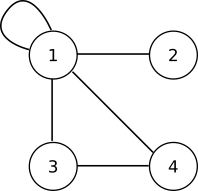
\includegraphics[width=0.15\paperwidth]{grafo}
\end{figure}

En esta imagen, hay cuatro elementos unidos a si mismos. Podemos ver que el 1 tiene enlaces con 1, 2, 3 y 4, el 2 solo tiene un enlace con 1, el 3 tiene enlace con 1 y 4 y el 4 tiene enlace con 1 y 3.

Cada uno de estos elementos puede representar un número, un caracter, un punto en 3D o cualquier cosa que deseas que representan, mientras que cada enlace puede tener un significado importante de ese elemento.

Es importante definir que cada enlace debe consistir en la unión de dos elementos, y estos elementos pueden ser el mismo (por ejemplo el enlace que esta unido al 1 dos veces).

\subsection{Nodos, ramas, hojas y raíces}

Se le conoce como nodo o vertice a cada elemento del grafo y se le conoce como rama, enlace o arista a cada enlace. En el ejemplo de arriba, podemos ver que existen cuatro nodos (1, 2, 3, 4) y cinco ramas (1:1, 1:2, 1:3, 1:4, 3:4).

En casos de ciertos grafos, es conveniente pensar que ciertos nodos son hojas o raices. Abajo hay dos ejemplos de grafos que presentan estos nodos con las hojas marcadas en azul y la raíz marcada en rojo

\begin{figure}[H]
    \centering
    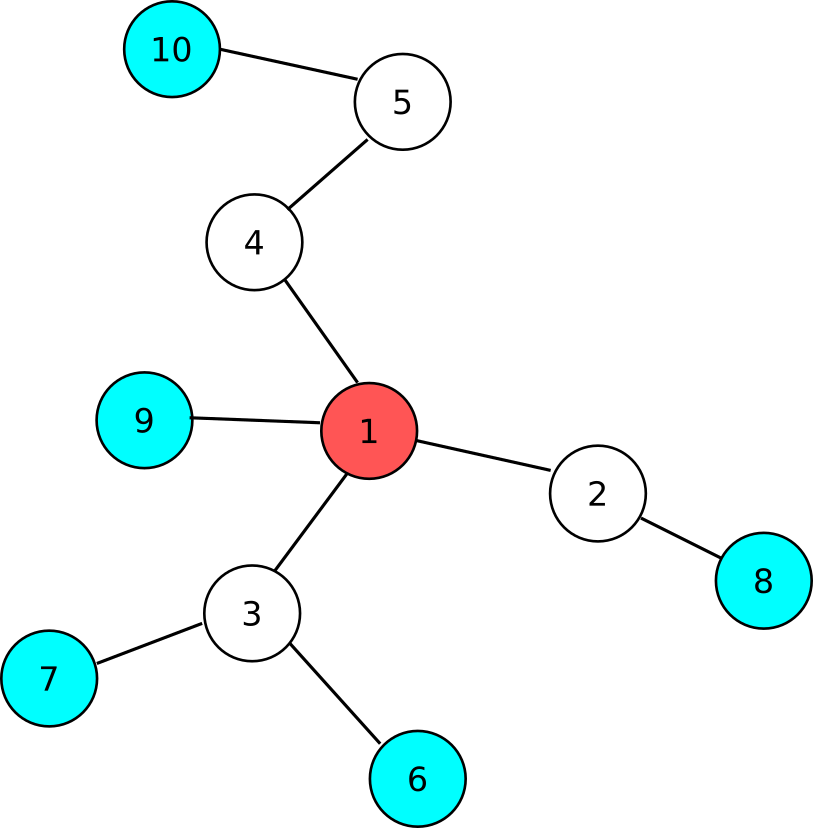
\includegraphics[width=0.25\paperwidth]{expansivo}
\end{figure}

\begin{figure}[H]
    \centering
    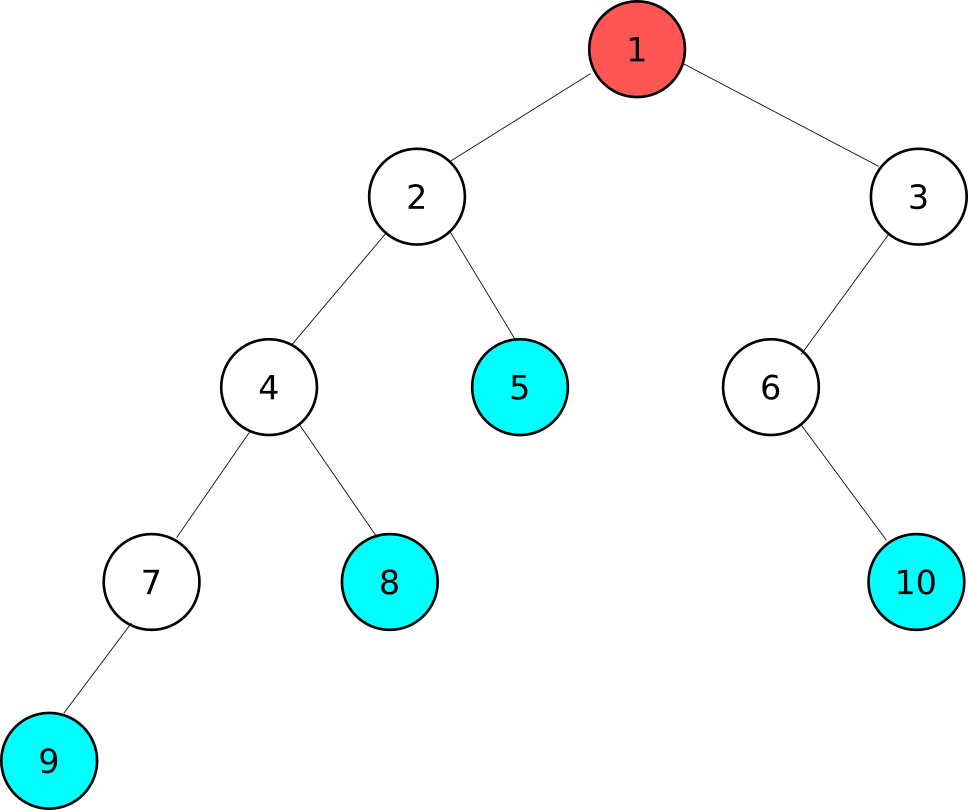
\includegraphics[width=0.3\paperwidth]{arbolbinario}
\end{figure}

Como se puede observar en ambos grafos, existe una raíz o nodo con la mayor cantidad de uniones y que es céntrico a todos los demás nodos, y existen varias hojas que se pueden considerar como nodos que estan en la orilla.

Cada nodo se puede considerar como "hijo" de otro nodo excepto la raíz, y cada nodo se puede considerar como "padre" de otro nodo excepto las hojas. En el primer grafo con la raíz y las hojas señaladas, se puede decir que 2, 3, 4 y 9 son hijos de 1 y que 1 es padre de 2, 3, 4 y 9.

Esta relación de padre y hijo es util será util después para optimizar operaciones relacionados con grafos.

\subsection{Grafos dirigidos y cíclicos}

Hasta ahorita hemos visto grafos no dirigidos, pero también existen grafos dirigidos que tienen ramas de un solo sentido:

\begin{figure}[H]
    \centering
    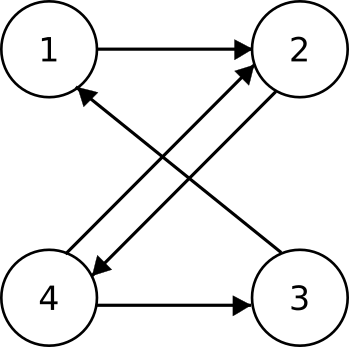
\includegraphics[width=0.15\paperwidth]{dirigido}
\end{figure}

Podemos ver que para llegar desde el nodo 1 al nodo 3 se tiene que pasar por los nodos 2 y 4 porque no hay un camino orientado hacia el nodo 3.

Un ejemplo de un grafo dirigido puede ser el mapa de todas las calles de un pueblo. En el pueblo, puede haber calles de doble sentido o calles de un solo sentido, y se puede representar cada calle como una rama.

Otra propiedad de los grafos ocurre cuando un grafo contiene un ciclo (es decir que puedes llegar a un mismo nodo pasando por ramas distintas en cada salto), entonces ese grafo puede ser considerado como cíclico.

Se puede observar que los dos grafos de la sección \textbf{Nodos, ramas, hojas y raíces} son acíclicos mientras que los otros dos son cíclicos.

\subsection{Grafos con pesos}

Muchas veces es conveniente darle pesos a las ramas de algún grafo para modificar la manera en la que se distribuyen los nodos. Digamos que quieres representar un país con N ciudades o nodos y quisieras saber cual es la mejor ruta de una ciudad a otra.

Para resolver este problema se puede considerar cada rama como una carretera de una ciudad a otra y se le puede poner un peso con la distancia real de esa carretera.

\begin{figure}[H]
    \centering
    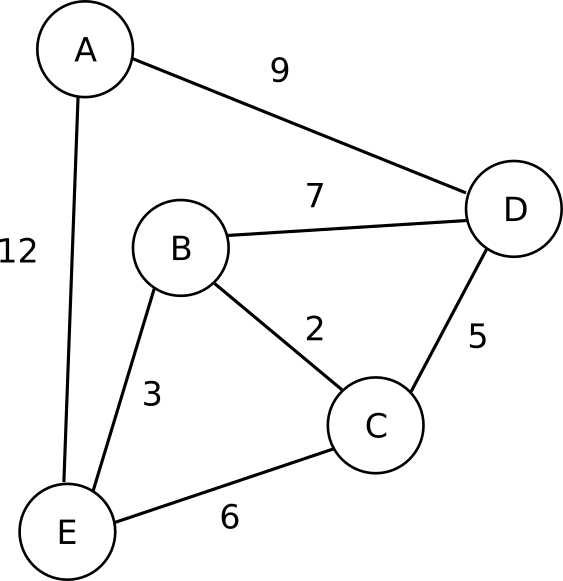
\includegraphics[width=0.2\paperwidth]{ciudades}
\end{figure}

Como se puede observar en el grafo de arriba, hay 5 ciudades (A, B, C, D, E) y varias carreteras con ciertas distancias (en este caso no nos importan las unidades).

Existen muchas posibles maneras de irse de la ciudad E y llegar a la ciudad D, pero solo hay un camino más optimo que los demás. Por ejemplo, podemos tomar el camino E - A - D, pero la suma de las distancias de cada carretera es de 12 + 9 o 21. La mejor opción es el camino de E - B - C - D con una suma total de 3 + 2 + 5 = 10. Se puede ver que a pesar de que se visitaron más nodos se recurrió menos distancia.

La siguiente sección cubre maneras de poder encontrar este camino más óptimo dado cualquier grafo.

\subsection{Arboles binarios}

Un arbol es un tipo de grafo que tiene una raíz en la parte de arriba que crece hacia abajo. Un arbol binario es una especie de arbol donde cada nodo tiene máximo dos hijos, el hijo izquierdo y el hijo derecho.

Este tipo de grafo es popular debido a que se pueden hacer operaciones eficientes sobre sus datos. Se puede implementar este tipo de grafo con un arreglo de tamaño $2^M$ donde M es la profundidad del arbol.

Para guardar un arbol en un arreglo, el primer elemento debe ser la raíz, luego los siguientes 2 elementos deben ser los hijos izquierdo y derecho de la raíz, luego los siguientes 4 elementos deben ser los hijos de esos hijos. Se debe repitir este proceso para llenar el arbol.

En caso de tener un nodo sin un hijo, se puede representar ese hijo con un valor especial.

Si tenemos un nodo en el índice $i$ del arreglo, sabemos que su hijo izquierdo tendría que estar en $2i + 1$ y su hijo derecho estaría en $2i + 2$. También sabemos que el padre de cualquier nodo siempre estará en el índice $\frac{i - 1}{2}$. Esta implementación simplifica la búsqueda de nodos.

\begin{figure}[H]
    \centering
    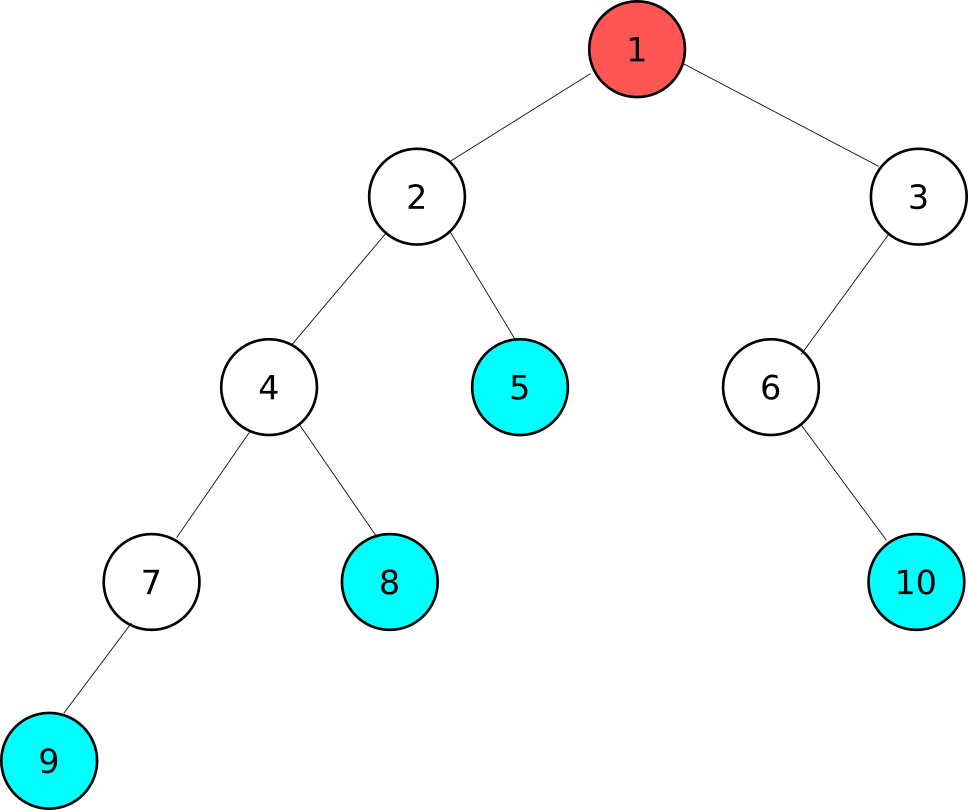
\includegraphics[width=0.3\paperwidth]{arbolbinario}
\end{figure}

Si quisieramos guardar el arbol de arriba en un arreglo de 10 elementos, tendríamos que definir un arreglo de $2^5$ elementos porque su profundidad es de 5. Si suponemos que cada espacio libre tiene valor -1, podemos representar este arbol con el siguiente arreglo: (1, 2, 3, 4, 5, 6, -1, 7, 8, -1, -1, -1, 10, -1, -1, 9).

Si queremos saber el hijo derecho del elemento en el índice 1 (nodo 2), podemos encontrarlo con la formula y se obtiene 2*1 + 2 = 4. Este elemento es el nodo 5 y se puede ver en la gráfica que el nodo 5 sí es el hijo derecho del nodo 2.

Podemos hacer búsquedas de nodos con el siguiente código:

\begin{lstlisting}[language=C++, caption=Arbol de binario]
#include <iostream>
#include <vector>

using namespace std;

int main() {
    vector<int> arbol = {1, 2, 3, 4, 5, 6, -1, 7, 8, -1, -1
    -1, 10, -1, -1, 9};
    cout << "Ingresa el numero de un nodo:" << endl;
    int nodoDeInteres;
    cin >> nodoDeInteres;
    int indice = -1;
    for(int i = 0; i < arbol.size(); i++) {
        if(nodoDeInteres == arbol[i]) {
            indice = i;
            break;
        }
    }
    if(indice == -1) {
        cout << "El nodo " << nodoDeInteres << " no es
        miembro de este arbol" << endl;
        return -1;
    }
    if(indice == 0) {
        cout << "Este nodo es la raiz, lo que significa que
        no tiene padre" << endl;
    } else {
        cout << "El padre del nodo " << nodoDeInteres <<
        "es el nodo " << arbol[(indice - 1) / 2] << endl;
    }
    int hijoIzquierdo = 2 * indice + 1;
    int hijoDerecho = 2 * indice + 2;
    if(hijoIzquierdo < arbol.size()) {
        if(arbol[hijoIzquierdo] != -1) {
            cout << "Su hijo izquierdo es el nodo " << arbol
            [hijoIzquierdo] << endl;
        } else {
            cout << "Este nodo no tiene hijo izquierdo"
            << endl;
        }
    } else {
        cout << "Este nodo no tiene hijo izquierdo" << endl;
    }
    if(hijoDerecho < arbol.size()) {
        if(arbol[hijoDerecho] != -1) {
            cout << "Su hijo derecho es el nodo " << arbol
            [hijoDerecho] << endl;
        } else {
            cout << "Este nodo no tiene hijo derecho"
            << endl;
        }
    } else {
        cout << "Este nodo no tiene hijo derecho" << endl;
    }
}
\end{lstlisting}
\href{https://repl.it/@Jamesscn/Arboles-Binarios}{Liga al código}

\subsection{Listas y matrices de adyacencia}

Para poder guardar grafos facilmente existen las listas y matrices de adyacencia. Una lista de adyacencia consiste en un arreglo de vectores donde cada nodo tiene un vector diciendo a que otros nodos esta conectado.

Digamos que tenemos el siguiente grafo y lo deseamos guardar en una lista de adyacencia:

\begin{figure}[H]
    \centering
    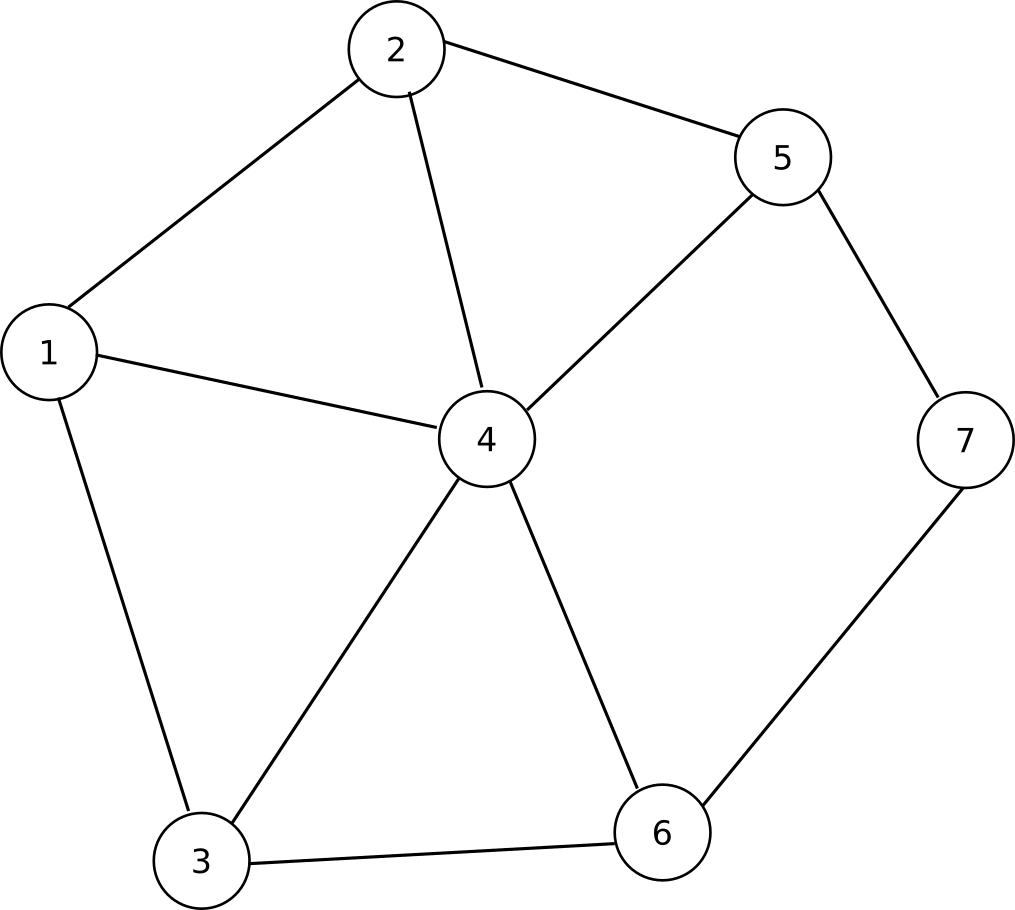
\includegraphics[width=0.32\paperwidth]{lista}
\end{figure}

Primero declararemos un arreglo de 7 vectores de enteros. Podemos ver que el nodo 1 esta conectado al nodo 2, 3 y 4 asi que guardaremos los valores 2, 3 y 4 en nuestro primer vector. Luego podemos ver que el nodo 2 esta conectado a 1, 4 y 5 asi que guardaremos los valores 1, 4 y 5 en nuestro segundo vector. Podemos repetir este proceso para todos los nodos y obtendremos lo siguiente:

1: [2, 3, 4]

2: [1, 4, 5]

3: [1, 4, 6]

4: [1, 2, 3, 5, 6]

5: [2, 4, 7]

6: [3, 4, 7]

7: [5, 6]

Estamos guardando 7 vectores porque el tamaño de cada uno puede variar. Este método es muy efectivo para guardar un grafo porque no consume mucho espacio y funciona para grafos dirigidos.

Sin embargo si un nodo tiene muchisimas ramas entonces la busqueda de una union entre dos nodos sería muy lento porque en el peor de los casos se tendrá que iterar sobre todos los ramas. Esto tiene complejidad de tiempo de O(E) y complejidad de espacio de O(E) donde E es la cantidad de ramas del grafo.

Si quisieramos mejorar nuestra complejidad de tiempo, tendríamos que empeorar nuestra complejidad de espacio. Para hacer esto podemos guardar el grafo en una matriz de adyacencia.

Una matriz de adyacencia consiste en un arreglo 2d de tamaño V * V donde V es la cantidad de vertices. En cada espacio, indicamos si hay o no hay una conexion entre cada nodo.

Para el ejemplo que habiamos dado antes, podemos crear la siguiente matriz donde un 0 significa que no hay conexión y un 1 significa que existe una rama entre esos dos nodos:

$$
\begin{bmatrix}
0 & 1 & 1 & 1 & 0 & 0 & 0 \\
1 & 0 & 0 & 1 & 1 & 0 & 0 \\
1 & 0 & 0 & 1 & 0 & 1 & 0 \\
1 & 1 & 1 & 0 & 1 & 1 & 0 \\
0 & 1 & 0 & 1 & 0 & 0 & 1 \\
0 & 0 & 1 & 1 & 0 & 0 & 1 \\
0 & 0 & 0 & 0 & 1 & 1 & 0 \\
\end{bmatrix}
$$

Por ejemplo, si quisieramos saber si las ramas 2 y 3 estan conectados podríamos checar la tercera columna de la segunda fila o la segunda columna de la tercera fila por un 1. Se debe notar que el matriz es simmetrico diagonalmente desde la esquina superior izquierda a la esquina inferior derecha para un grafo no dirigido.

Como se puede observar, disminuimos la complejidad de tiempo a O(1) pero aumentamos la complejidad de espacio a O($V^2$).

Otra ventaja de usar una matriz de adyacencia es que se puede guardar un grafo con pesos facilmente reemplazando los 1s con el peso de cada rama, mientras que con una lista de adyacencia se tendría que tener otra estrategia como guardar los pesos en una estructura.

\begin{figure}[H]
    \centering
    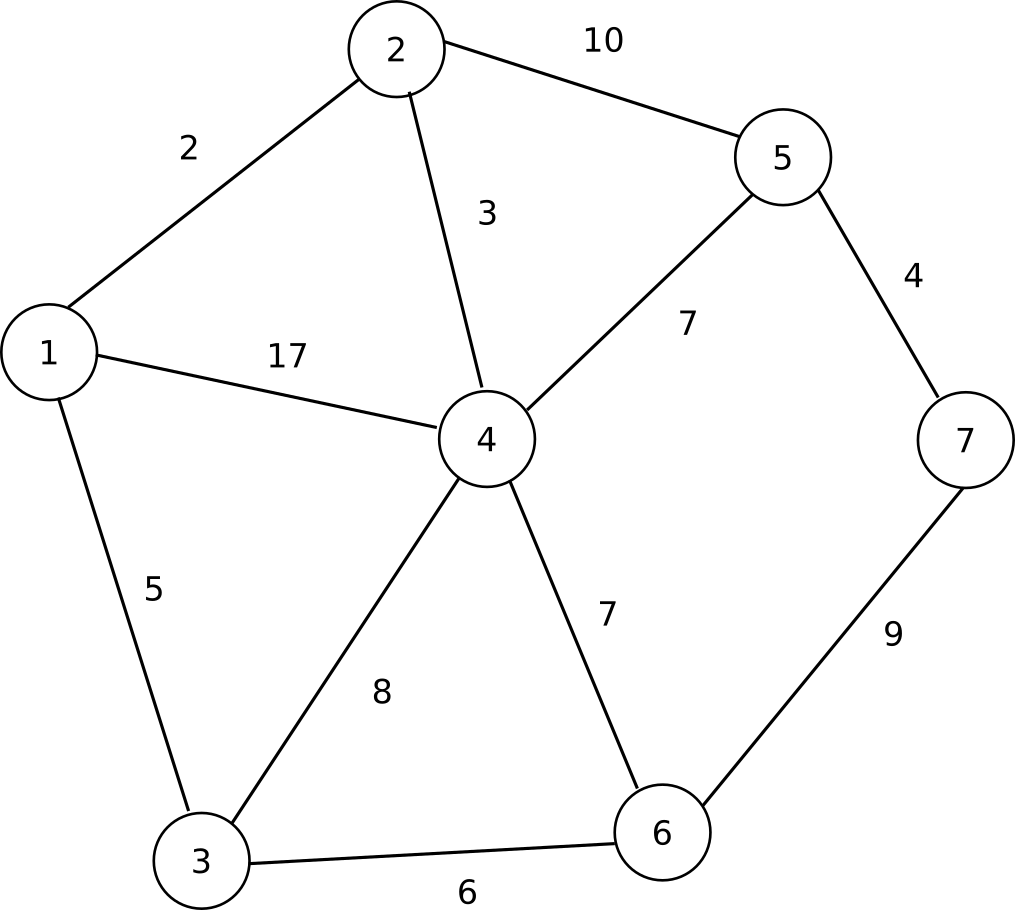
\includegraphics[width=0.32\paperwidth]{dijkstra}
\end{figure}

Si quisieramos guardar el último grafo con pesos, esta sería su matriz:

$$
\begin{bmatrix}
0 & 2 & 5 & 17 & 0 & 0 & 0 \\
2 & 0 & 0 & 3 & 10 & 0 & 0 \\
5 & 0 & 0 & 8 & 0 & 6 & 0 \\
17 & 3 & 8 & 0 & 7 & 7 & 0 \\
0 & 10 & 0 & 7 & 0 & 0 & 4 \\
0 & 0 & 6 & 7 & 0 & 0 & 9 \\
0 & 0 & 0 & 0 & 4 & 9 & 0 \\
\end{bmatrix}
$$

\subsection{Grafos con arreglos 2D}

Los problemas de grafos más comunes y más faciles tienden a ser esos que ocurren en un plano 2D y que pueden ser representados sobre un arreglo 2D.

Un ejemplo común es pensar en un plano como la vista superficial de un laberinto, y construir un arreglo bidimensional de booleanos donde verdadero es una pared u obstaculo y falso es un camino libre.

Aqui hay un ejemplo donde cada 1 se ha pintado de negro y cada 0 se ha dejado en blanco:

\begin{figure}[H]
    \centering
    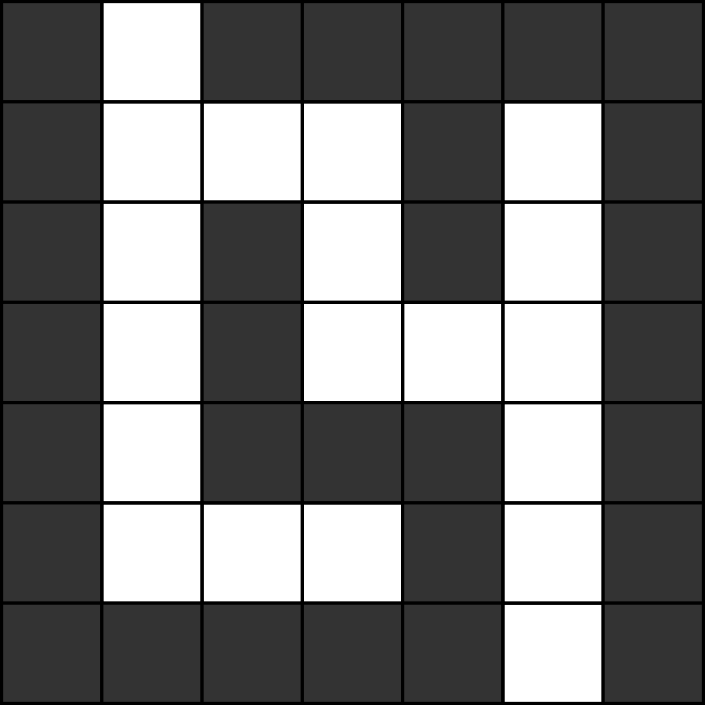
\includegraphics[width=0.2\paperwidth]{grafo2d}
\end{figure}

Si asumimos que somos una persona que esta resolviendo este laberinto y queremos encontrar un camino desde la esquina superior izquierda a la esquina inferior derecha, y solo podemos movernos en cuatro direcciones (arriba, abajo, izquierda o derecha), entonces podemos pensar en este problema como un especie de grafo que podemos resolver.

Ahora hablaremos de como resolver este tipo de problema.

\section{Algoritmos de búsqueda}

Los algoritmos de búsqueda son métodos especiales de encontrar el camino más corto entre dos nodos de un grafo. Esto tiene muchas aplicaciones, como encontrar la ruta más rapida entre dos ciudades o encontrar la solución a un laberinto.

\subsection{Algoritmos heuristicos o greedy}

Se le denota algoritmo greedy a cualquier tipo de algoritmo que toma la decisión más conveniente en todos los pasos de un conjunto de decisiones.

Podemos demostrar este concepto facilmente con el siguiente laberinto:

\begin{figure}[H]
    \centering
    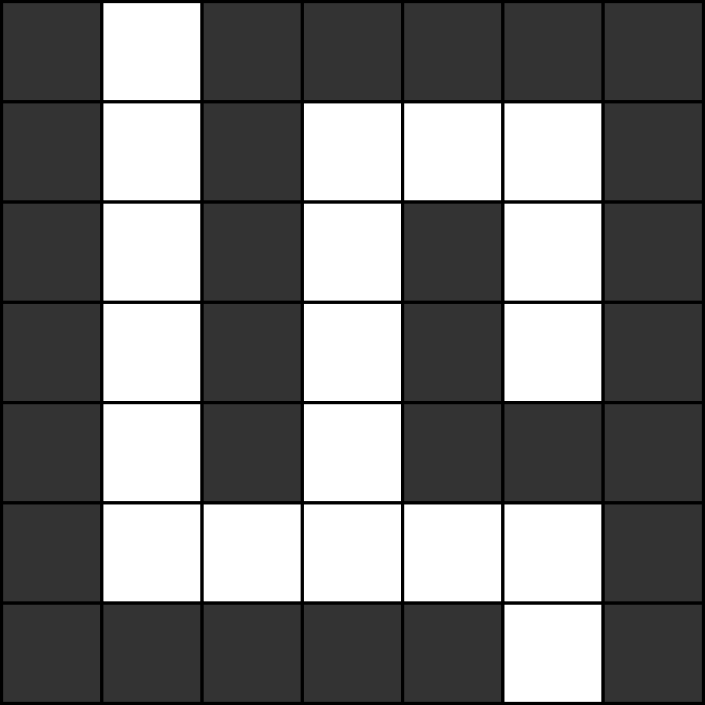
\includegraphics[width=0.2\paperwidth]{greedy}
\end{figure}

Como sabemos que la salida del laberinto siempre estará a nuestra derecha y hacia abajo, entonces un algoritmo greedy nos dirá que siempre debemos mover en una de estas dos direcciones dependiendo de donde estemos.

Primero iniciamos en el primer espacio y solo podemos movernos abajo asi que tomamos esa ruta, luego en el segundo espacio podemos movernos para arriba denuevo o abajo. Decidimos movernos para abajo porque sabemos que la salida está más abajo.

Seguimos esto hasta llegar a la esquina inferior izquierda, y entonces nos empezamos a mover hacia la derecha en lugar de arriba o denuevo a la izquierda porque sabemos que la meta sigue estando a la derecha.

Podemos hacer un programa que prioritiza moverse hacia abajo cuando la meta esta más para abajo que a la izquierda y que prioritiza moverse más para la derecha en caso contrario.

\begin{lstlisting}[language=C++, caption=Camino greedy]
#include <iostream>
#include <utility>

using namespace std;

int main() {
    bool mapa[][7] = {
        {1, 0, 1, 1, 1, 1, 1},
        {1, 0, 1, 0, 0, 0, 1},
        {1, 0, 1, 0, 1, 0, 1},
        {1, 0, 1, 0, 1, 0, 1},
        {1, 0, 1, 0, 1, 1, 1},
        {1, 0, 0, 0, 0, 0, 1},
        {1, 1, 1, 1, 1, 0, 1}};
    pair<int, int> puntoActual = make_pair(1, 0);
    pair<int, int> puntoFinal = make_pair(5, 6);
    int iteracion = 0;
    while(puntoActual.first != puntoFinal.first || puntoActual.second != puntoFinal.second) {
        int x = puntoActual.first;
        int y = puntoActual.second;
        int distanciaX = puntoFinal.first - x;
        int distanciaY = puntoFinal.second - y;
        if(distanciaX > distanciaY) {
            if(mapa[y][x + 1] == 0) {
                puntoActual = make_pair(x + 1, y);
            } else if (mapa[y + 1][x] == 0) {
                puntoActual = make_pair(x, y + 1);
            } else {
                cout << "No se pudo llegar a la meta" << endl;
                return 0;
            }
        } else {
            if(mapa[y + 1][x] == 0) {
                puntoActual = make_pair(x, y + 1);
            } else if (mapa[y][x + 1] == 0) {
                puntoActual = make_pair(x + 1, y);
            } else {
                cout << "No se pudo llegar a la meta" << endl;
                return 0;
            }
        }
        cout << "Iteracion #" << iteracion << endl;
        for(int j = 0; j < 7; j++) {
            for(int i = 0; i < 7; i++) {
                if(i == puntoActual.first && j == puntoActual.second) {
                    cout << "x";
                } else if (mapa[j][i] == 1) {
                    cout << "#";
                } else {
                    cout << " ";
                }
            }
            cout << endl;
        }
        cout << endl;
        iteracion++;
    }
}
\end{lstlisting}
\href{https://repl.it/@Jamesscn/Algoritmos-Greedy}{Liga al código} \\

Si corremos el código, podemos ver que se encuentra una solución señalada en la grafica de abajo en azúl:

\begin{figure}[H]
    \centering
    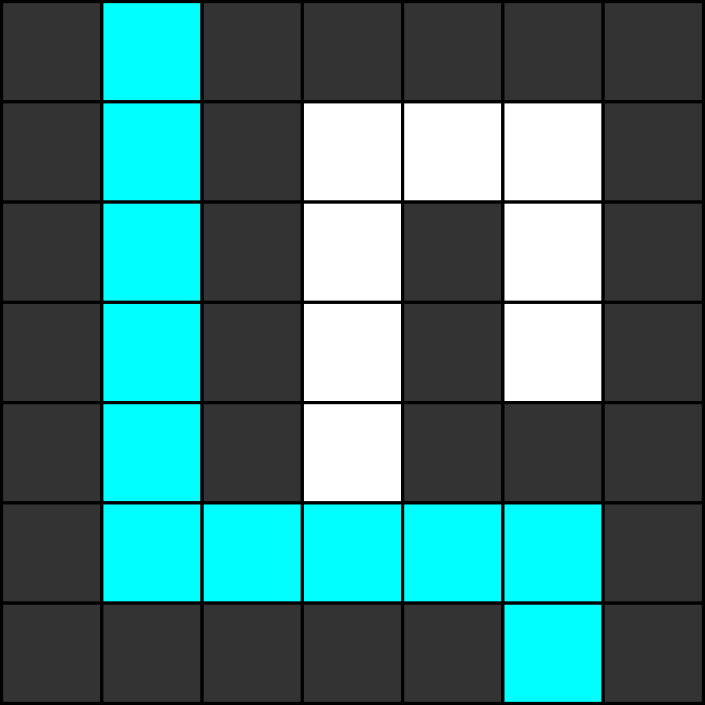
\includegraphics[width=0.2\paperwidth]{greedybueno}
\end{figure}

Pero existen varias desventajas con los algoritmos greedy, particularmente cuando hay caminos que no van a ningun lado. Si hacemos una pequeña modificación al mapa, podemos ver que el algoritmo se atora y no llega a la meta:

\begin{figure}[H]
    \centering
    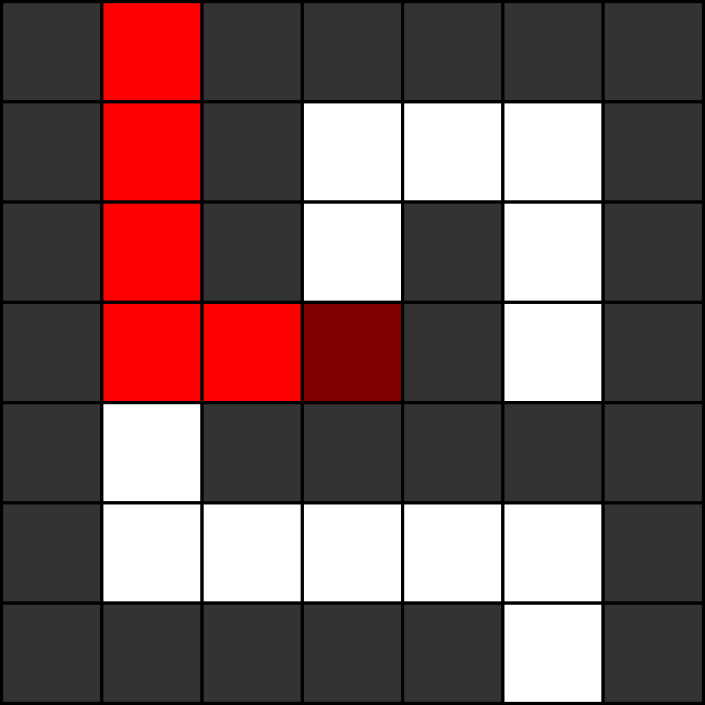
\includegraphics[width=0.2\paperwidth]{greedymalo}
\end{figure}

Esto es porque cuando el algoritmo llegó al cuarto espacio tuvo una decisión de moverse hacia abajo o hacia la derecha. Como el algoritmo piensa que es mejor irse moviendo a la derecha porque la meta esta más a la derecha que abajo, toma un camino falso y se atora.

Se debe observar que en este caso no lo hemos programado para que siga moviendose en caso de haber pared abajo y a la derecha. Esto es porque podría atorarse en un ciclo infinito donde parece que se esta avanzando a la meta pero nunca llega.

Este concepto de heuristica donde se sigue el "instinto" de programa es bueno en ciertos casos, pero no se debe tomar puras decisiones basados en instinto.

\subsection{Búsqueda en anchura}

Para poder encontrar el camino correcto, se deben simular distintos caminos para encontrar la más rapida. La búsqueda en anchura esta garantizado a dar el camino más corto entre dos nodos para cualquier grafo sin pesos.

La búsqueda en anchura también se conoce como breadth first search o simplemente \textbf{BFS} en íngles y es bastante popular.

Este método inicia checando todos bloques al rededor del inicio, luego los espacios al rededor de esos hasta llegar a la meta. Este método puede ser algo ineficiente debido a la gran cantidad de espacios que se tendrán que checar, pero no es muy dificil de programar.

En la siguiente figura, se puede ver un ejemplo de como se expande una búsqueda en anchura con el número de cada iteración marcado con un número. Primero se inicia en el lugar uno y se marcan todos los espacios a su alrededor con un dos, luego se marcan los espacios alrededor del dos que no fueron visitados con tres y se repite hasta llegar al final.

\begin{figure}[H]
    \centering
    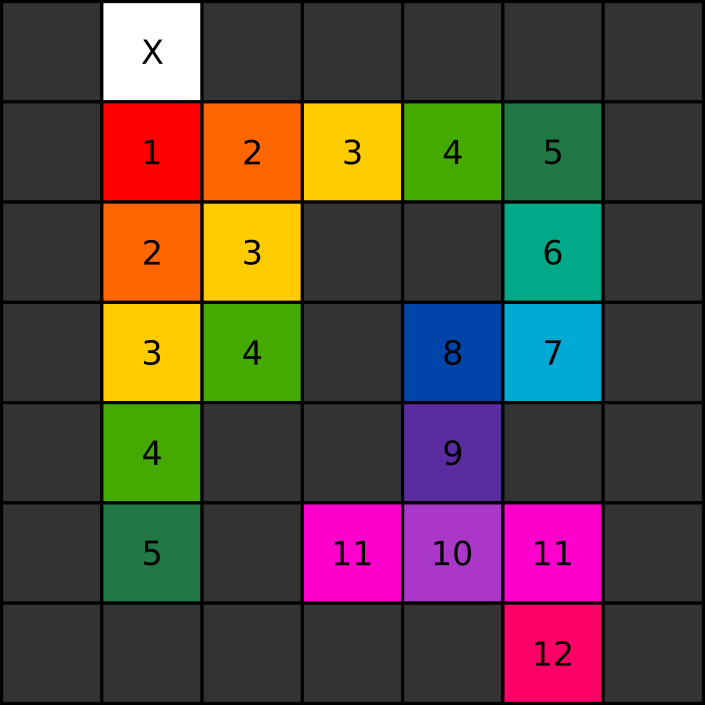
\includegraphics[width=0.3\paperwidth]{bfs}
\end{figure}

Cada vez que se llega a un lugar nuevo, este se marca con algo para indicar que ya fue visitado y para evitar que el programa nunca termine. 

Hasta ahorita, se han marcado todos los espacios libres del grafo con números pero no se ha definido cual es el camino más corto, sino que el mínimo número de pasos para llegar a la meta.

Si quisieramos saber cual es el camino más corto, se tendrá que iniciar desde la meta y contar los números para abajo hasta llegar al inicio. Podemos imaginar los números como flechas que indican a que bloque uno se debe mover para estar un paso más cerca a la entrada.

\begin{figure}[H]
    \centering
    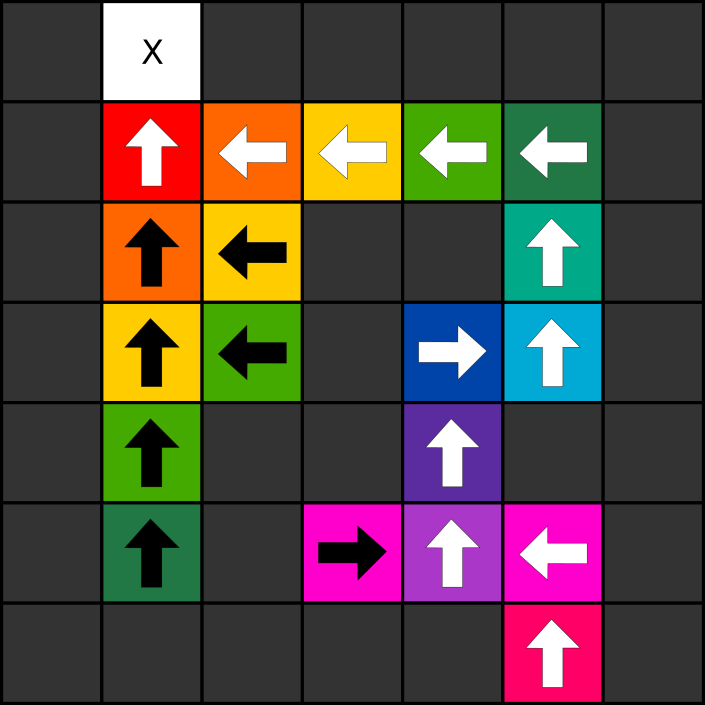
\includegraphics[width=0.3\paperwidth]{bfscamino}
\end{figure}

De esta manera podemos obtener el camino de regreso. Un método más conveniente de hacer este proceso es guardar la X y la Y de cada bloque cuando se salta a uno nuevo en la primera fase para no tener que buscar un número más pequeño en cada iteración.

Para implementar este algoritmo se pueden usar structs para guardar los datos de cada espacio (Si se ha visitado este lugar, su X y Y, la X y Y del último bloque que fue visitado). Además se debe tener una fila o queue para ir almacenando todos los espacios que estan pendientes de revisar.

Después de cada iteración, se debe eliminar el último lugar que fue visitado de la fila y se deben agregar todos los lugares adjacentes que no se han visitado. Esta es la implementación:

\begin{lstlisting}[language=C++, caption=Búsqueda en anchura]
#include <iostream>
#include <queue>
#include <vector>

using namespace std;

struct Punto {
    int x;
    int y;
    int ultimoX;
    int ultimoY;
    bool visitado;
};

int main() {
    bool mapa[][7] = {
        {1, 0, 1, 1, 1, 1, 1},
        {1, 0, 0, 0, 0, 0, 1},
        {1, 0, 0, 1, 1, 0, 1},
        {1, 0, 0, 1, 0, 0, 1},
        {1, 0, 1, 1, 0, 1, 1},
        {1, 0, 1, 0, 0, 0, 1},
        {1, 1, 1, 1, 1, 0, 1}};
    Punto puntos[7][7];
    for(int y = 0; y < 7; y++) {
        for(int x = 0; x < 7; x++) {
            puntos[y][x].x = x;
            puntos[y][x].y = y;
            puntos[y][x].visitado = false;
        }
    }
    int xInicial = 1;
    int yInicial = 0;
    int xFinal = 5;
    int yFinal = 6;
    //Iniciar la busqueda con el punto inicial
    queue<Punto> bfs;
    bfs.push(puntos[yInicial][xInicial]);
    puntos[yInicial][xInicial].visitado = true;
    while(bfs.size() > 0) {
        Punto actual = bfs.front();
        bfs.pop();
        int x = actual.x;
        int y = actual.y;
        //Checar si los puntos adyacentes no estan fuera del arreglo y agregarlos a la fila si no han sido visitados
        if(x + 1 < 7) {
            if(puntos[y][x + 1].visitado == false && mapa[y][x + 1] == false) {
                bfs.push(puntos[y][x + 1]);
                puntos[y][x + 1].visitado = true;
                puntos[y][x + 1].ultimoX = x;
                puntos[y][x + 1].ultimoY = y;
            }
        }
        if(x - 1 >= 0) {
            if(puntos[y][x - 1].visitado == false && mapa[y][x - 1] == false) {
                bfs.push(puntos[y][x - 1]);
                puntos[y][x - 1].visitado = true;
                puntos[y][x - 1].ultimoX = x;
                puntos[y][x - 1].ultimoY = y;
            }
        }
        if(y + 1 < 7) {
            if(puntos[y + 1][x].visitado == false && mapa[y + 1][x] == false) {
                bfs.push(puntos[y + 1][x]);
                puntos[y + 1][x].visitado = true;
                puntos[y + 1][x].ultimoX = x;
                puntos[y + 1][x].ultimoY = y;
            }
        }
        if(y - 1 >= 0) {
            if(puntos[y - 1][x].visitado == false && mapa[y - 1][x] == false) {
                bfs.push(puntos[y - 1][x]);
                puntos[y - 1][x].visitado = true;
                puntos[y - 1][x].ultimoX = x;
                puntos[y - 1][x].ultimoY = y;
            }
        }
    }
    vector<Punto> camino;
    Punto actual = puntos[yFinal][xFinal];
    while(actual.x != xInicial || actual.y != yInicial) {
        camino.push_back(actual);
        actual = puntos[actual.ultimoY][actual.ultimoX];
    }
    cout << "El camino es: " << endl;
    for(int i = camino.size() - 1; i >= 0; i--) {
        cout << camino[i].x << ", " << camino[i].y << endl;
    }
}
\end{lstlisting}
\href{https://repl.it/@Jamesscn/Busqueda-en-Anchura}{Liga al código} \\

Al correr este código, se debe obtener una lista de puntos que consiste en el camino más corto a la meta.

\subsection{Búsqueda en profundidad}

La búsqueda en profundidad es conocida como depth first search o \textbf{DFS} en íngles trabaja de una manera distinta a la búsqueda en anchura. En lugar de expandir su busqueda por niveles, recorre un camino hasta llegar a un lugar sin salida y se regresa al último espacio donde había una decisión.

Si un humano tuviera que recorrer un laberinto lo mas probable es que usaría este método para encontrar la salida ya que estaría marcando todas las zonas sin salida y probando zonas nuevas. No podrá hacerlo usando BFS porque eso implicaría que tendría que teletransportarse de un lugar a otro.

Se puede ver en la siguiente figura todos los caminos que se tendrán que recorrer hasta llegar al final:

\begin{figure}[H]
    \centering
    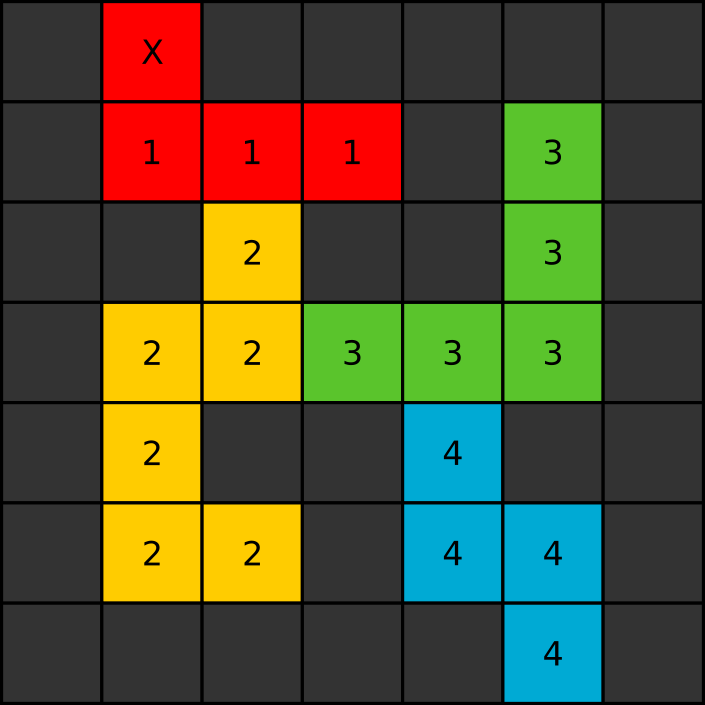
\includegraphics[width=0.3\paperwidth]{dfs}
\end{figure}

En este caso el algoritmo prioritiza primero los caminos hacia arriba, luego los de la izquierda, luego los de la derecha y finalmente los de abajo. El algoritmo va a recorrer el camino 1 y al llegar al final del camino se regresa un espacio y prueba el camino 2 de abajo. Luego como no hay salida en el camino 2 prueba el 3 y finalmente el 4.

Para poder encontrar el camino, se debe marcar el ultimo bloque que fue visitado al igual que con BFS y se debe recorrer este camino empezando desde la salida.

Si queremos implementar este algoritmo, debemos guardar cada posición que se desea buscar en una pila o stack y seguir la búsqueda hasta llegar a la salida o hasta que se vacie la pila.

Si vemos la implementación de este algoritmo podemos observar que es exactamente igual al código de BFS con el único cambio de que ahora se esta usando un stack en lugar de un queue:

\begin{lstlisting}[language=C++, caption=Búsqueda en anchura]
#include <iostream>
#include <stack>
#include <vector>

using namespace std;

struct Punto {
    int x;
    int y;
    int ultimoX;
    int ultimoY;
    bool visitado;
};

int main() {
    bool mapa[][7] = {
        {1, 0, 1, 1, 1, 1, 1},
        {1, 0, 0, 0, 0, 0, 1},
        {1, 0, 0, 1, 1, 0, 1},
        {1, 0, 0, 1, 0, 0, 1},
        {1, 0, 1, 1, 0, 1, 1},
        {1, 0, 1, 0, 0, 0, 1},
        {1, 1, 1, 1, 1, 0, 1}};
    Punto puntos[7][7];
    for(int y = 0; y < 7; y++) {
        for(int x = 0; x < 7; x++) {
            puntos[y][x].x = x;
            puntos[y][x].y = y;
            puntos[y][x].visitado = false;
        }
    }
    int xInicial = 1;
    int yInicial = 0;
    int xFinal = 5;
    int yFinal = 6;
    //Iniciar la busqueda con el punto inicial
    stack<Punto> dfs;
    dfs.push(puntos[yInicial][xInicial]);
    puntos[yInicial][xInicial].visitado = true;
    while(dfs.size() > 0) {
        Punto actual = dfs.top();
        dfs.pop();
        int x = actual.x;
        int y = actual.y;
        //Checar si los puntos adyacentes no estan fuera del arreglo y agregarlos a la fila si no han sido visitados
        if(x + 1 < 7) {
            if(puntos[y][x + 1].visitado == false && mapa[y][x + 1] == false) {
                dfs.push(puntos[y][x + 1]);
                puntos[y][x + 1].visitado = true;
                puntos[y][x + 1].ultimoX = x;
                puntos[y][x + 1].ultimoY = y;
            }
        }
        if(x - 1 >= 0) {
            if(puntos[y][x - 1].visitado == false && mapa[y][x - 1] == false) {
                dfs.push(puntos[y][x - 1]);
                puntos[y][x - 1].visitado = true;
                puntos[y][x - 1].ultimoX = x;
                puntos[y][x - 1].ultimoY = y;
            }
        }
        if(y + 1 < 7) {
            if(puntos[y + 1][x].visitado == false && mapa[y + 1][x] == false) {
                dfs.push(puntos[y + 1][x]);
                puntos[y + 1][x].visitado = true;
                puntos[y + 1][x].ultimoX = x;
                puntos[y + 1][x].ultimoY = y;
            }
        }
        if(y - 1 >= 0) {
            if(puntos[y - 1][x].visitado == false && mapa[y - 1][x] == false) {
                dfs.push(puntos[y - 1][x]);
                puntos[y - 1][x].visitado = true;
                puntos[y - 1][x].ultimoX = x;
                puntos[y - 1][x].ultimoY = y;
            }
        }
    }
    vector<Punto> camino;
    Punto actual = puntos[yFinal][xFinal];
    while(actual.x != xInicial || actual.y != yInicial) {
        camino.push_back(actual);
        actual = puntos[actual.ultimoY][actual.ultimoX];
    }
    cout << "El camino es: " << endl;
    for(int i = camino.size() - 1; i >= 0; i--) {
        cout << camino[i].x << ", " << camino[i].y << endl;
    }
}
\end{lstlisting}
\href{https://repl.it/@Jamesscn/Busqueda-en-Profundidad}{Liga al código} \\

Debido a su similaridad ambas búsquedas se tardarán practicamente lo mismo en el peor de los casos.

\subsection{Algoritmo de Dijsktra}

Para grafos con pesos BFS y DFS no son capaces de encontrar el camino menos pesado entre dos nodos, asi que se debe utilizar el algoritmo de Dijkstra en esos casos.

El algoritmo de Dijkstra consiste en encontrar el nodo con menor distancia que no ha sido visitado y a partir de ese nodo se debe calcular si la distancia a otros nodos es menor a la distancia que esos nodos tenian antes. En caso de sí ser menor, entonces se debe marcar el nodo previo para guardar el camino.

Se mostrará un ejemplo usando la siguiente figura:

\begin{figure}[H]
    \centering
    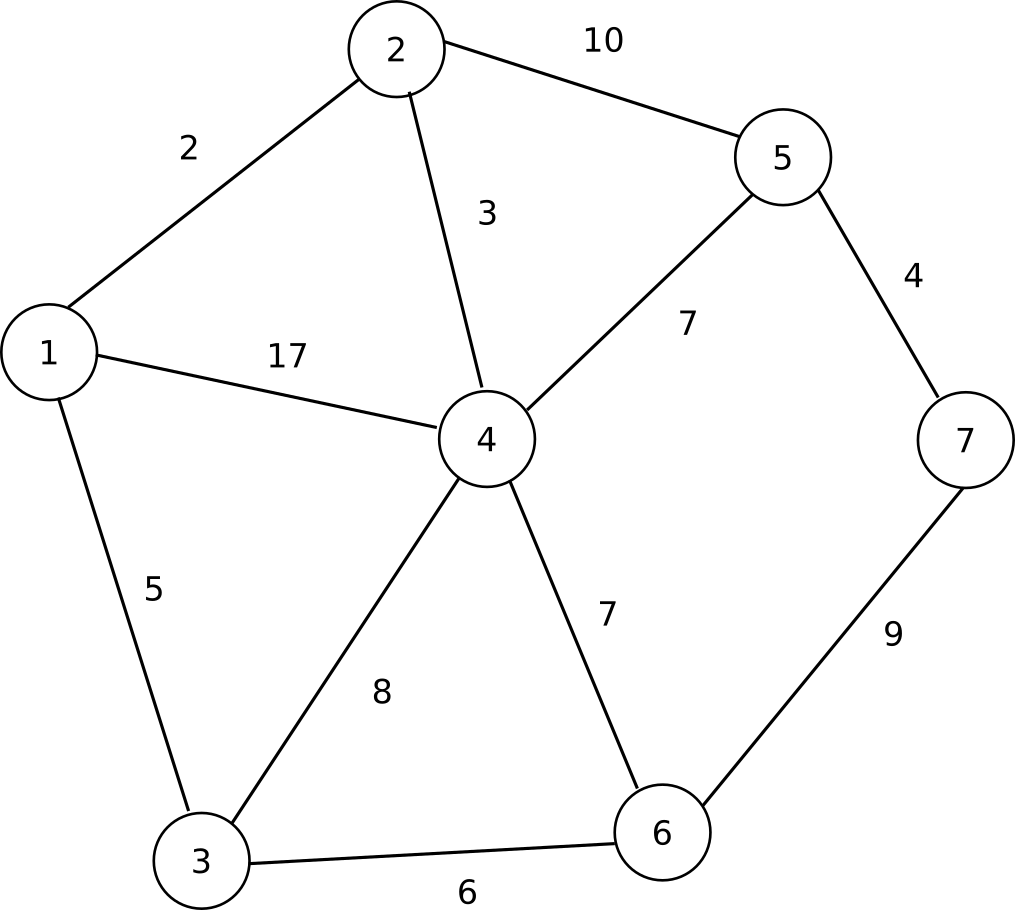
\includegraphics[width=0.4\paperwidth]{dijkstra}
\end{figure}

Digamos que queremos encontrar el camino menos pesado del nodo 1 al nodo 7. Para hacer esto inicialmente se le debe de asignar a todos los nodos una distancia desde el nodo 1 de infinito. El nodo 1 debe tener una distancia de 0 porque es el mismo nodo. Ahora se buscará el nodo con distancia menor no marcado (en este caso 1 con distancia 0) y se debe de calcular las sumas de las distancias desde ese nodo a sus conexiones.

Como hay tres ramas hay tres sumas, 0 + 2 = 2 para el nodo 2, 0 + 5 = 5 para el nodo 3 y 0 + 17 = 17 para el nodo 4. Como estos tres distancias son menores a la distancia que originalmente tenian (infinito), entonces esas distancias reemplazan las originales.

Como ya se vieron todas las conexiones del nodo 1, se debe guardar el nodo 1 como marcado.

Ahora se debe buscar el siguiente nodo más pequeño no visitado (en este caso el nodo 2 con distancia 2) y se debe repetir el proceso hasta que no se pueda hacer más búsquedas.

Se ha marcado la siguiente gráfica con el camino menos pesado en rojo y las distancias mínimas a cada nodo en azul:

\begin{figure}[H]
    \centering
    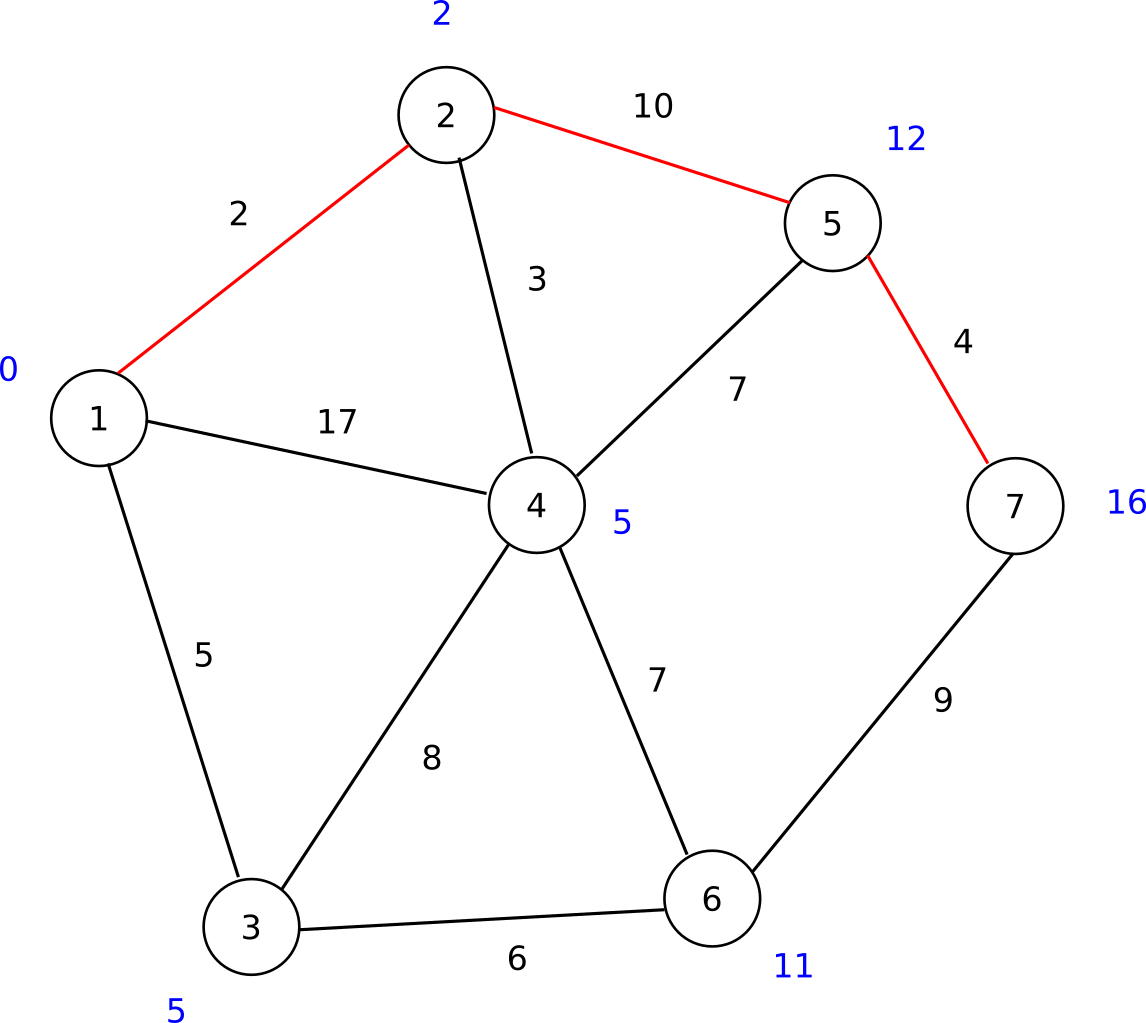
\includegraphics[width=0.42\paperwidth]{dijkstracamino}
\end{figure}

El siguiente código implementa el algoritmo para resolver este caso considerando que 2147483647 es infinito:

\begin{lstlisting}[language=C++, caption=Algoritmo de Dijkstra]
#include <iostream>

using namespace std;

int main() {
    int grafo[][7] = {{-1,  2,  5, 17, -1, -1, -1},
                        { 2, -1, -1,  3, 10, -1, -1},
                        { 5, -1, -1,  8, -1,  6, -1},
                        {17,  3,  8, -1,  7,  7, -1},
                        {-1, 10, -1,  7, -1, -1,  4},
                        {-1, -1,  6,  7, -1, -1,  9},
                        {-1, -1, -1, -1,  4,  9, -1}};
    int distancias[7];
    int previo[7];
    bool marcados[7];
    distancias[0] = 0;
    marcados[0] = false;
    for(int i = 1; i < 7; i++) {
        distancias[i] = 2147483647;
        marcados[i] = false;
    }
    while(true) {
        int minimo = -1;
        for(int i = 0; i < 7; i++) {
            if(!marcados[i]) {
                if(minimo == -1) {
                    minimo = i;
                }
                if(distancias[i] < distancias[minimo] &&
                distancias[i] != 2147483647) {
                    minimo = i;
                }
            }
        }
        if(minimo == -1) {
            break;
        }
        marcados[minimo] = true;
        for(int i = 0; i < 7; i++) {
            if(!marcados[i] && grafo[minimo][i] != -1) {
                int distanciaNueva = distancias[minimo] + grafo[minimo][i];
                if(distanciaNueva < distancias[i]) {
                    distancias[i] = distanciaNueva;
                    previo[i] = minimo;
                }
            }
        }
    }
    int actual = 6;
    while(actual != 0) {
        cout << actual + 1 << " <=> ";
        actual = previo[actual];
    }
    cout << 1 << endl;
    cout << "Distancia minima: " << distancias[6] << endl;
}
\end{lstlisting}
\href{https://repl.it/@Jamesscn/Algoritmo-de-Dijkstra}{Liga al código} \\

Además de Dijkstra, existen otros algoritmos que son más eficientes en diferentes casos, como el algoritmo de Floyd-Warshall y el algoritmo de Johnson.

\subsection{A*}

Mientras que se puede simular todos los caminos para encontrar el más corto este proceso es lento, y el proceso de usar el "instinto" o la heuristica tiende a encontrar un camino muy rapido pero este no es el más corto.

El algoritmo A* mezcla estos dos conceptos para crear un algoritmo que siempre encontrará el camino corto entre dos nodos en casi el mismo tiempo que el algoritmo heuristico. Este algoritmo es muy eficiente, sin embargo solo sirve para encontrar el camino a una meta mientras que algún algoritmo como Dijkstra o BFS puede encontrar el camino menos pesado a todos los nodos como conjunto en menos tiempo. Este algoritmo es muy popular en los videojuegos para crear enemigos que persiguen al jugador.

Como A* se basa en la heuristica, puede suceder que encuentre un camino muy parecido al menos pesado pero no el menos pesado. Para garantizar que siempre encontrará el mejor camino se debe usar una función de heuristica "admisible" o siempre debe tener una idea de la distancia exacta entre dos nodos.

Para poder implementar este algoritmo, se debe buscar todos los nodos al rededor de la inicial y calcular su costo de movimiento. Cada costo de movimiento será la suma del peso de la rama al otro nodo y la distancia heuristica desde ese nodo a la meta.

Si estamos trabajando con arreglo 2D donde nos podemos mover en solo 4 direcciones sin pesos entonces la suma solo sería la suma de los valores absolutos de las distancias a la meta. Si estamos trabajando con un arreglo 2D donde podemos movernos en 8 direcciones, podemos pensar que cada movimiento horizontal o vertical tiene una distancia de 1 y cada movimiento diagonal tiene una distancia de $\sqrt{2}$ o 1.414.

En la siguiente gráfica se encontró el camino más corto utilizando A* asumiendo que solo se puede mover en los 4 direcciones:

\begin{figure}[H]
    \centering
    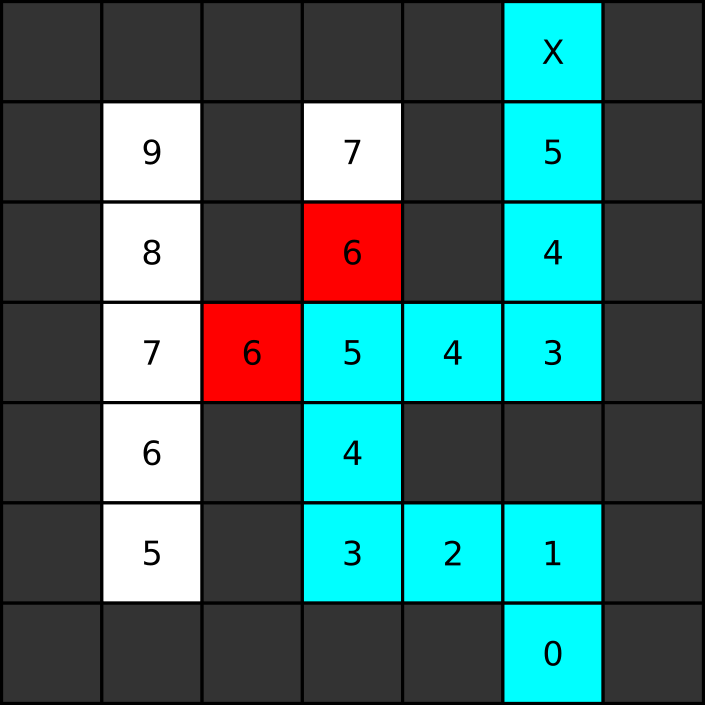
\includegraphics[width=0.32\paperwidth]{astrella}
\end{figure}

Se han marcado todas las distancias como la suma de los valores absoluto de las distancias en X y Y a la meta y en cada iteración siempre se escoge el camino con el número más pequeño que no ha sido visitado.

Luego se debe marcar el último nodo que fue visitado al igual que todos los demás algoritmos de búsqueda para poder encontrar el camino correcto.

Si deseamos verlo en C++, podemos usar una fila de prioridad para obtener el punto con menos distancia que se ha buscado:

\begin{lstlisting}[language=C++, caption=A*]
#include <iostream>
#include <vector>
#include <queue>
#include <cmath>

using namespace std;

struct Punto {
    int x;
    int y;
    int distancia;
    bool visitado;
};

//Es necesario para ordenar los datos en la fila
struct ComparaDistancia {
    bool operator()(Punto const& p1, Punto const& p2) {
        return p1.distancia > p2.distancia;
    }
};

int main() {
    int grafo[][7] = {{1, 1, 1, 1, 1, 0, 1},
                        {1, 0, 1, 0, 1, 0, 1},
                        {1, 0, 1, 0, 1, 0, 1},
                        {1, 0, 0, 0, 0, 0, 1},
                        {1, 0, 1, 0, 1, 1, 1},
                        {1, 0, 1, 0, 0, 0, 1},
                        {1, 1, 1, 1, 1, 0, 1}};
    Punto puntos[7][7];
    for(int y = 0; y < 7; y++) {
        for(int x = 0; x < 7; x++) {
            puntos[y][x].x = x;
            puntos[y][x].y = y;
            puntos[y][x].visitado = false;
        }
    }
    int xInicial = 5;
    int yInicial = 0;
    int xFinal = 5;
    int yFinal = 6;
    priority_queue<Punto, vector<Punto>, ComparaDistancia> camino;
    Punto inicial = puntos[yInicial][xInicial];
    inicial.distancia = 6;
    inicial.visitado = true;
    camino.push(inicial);
    while(camino.size() > 0) {
        Punto actual = camino.top();
        camino.pop();
        int x = actual.x;
        int y = actual.y;
        cout << x << ", " << y << endl;
        if(x == xFinal && y == yFinal) {
            break;
        }
        if(x - 1 >= 0) {
            if(!puntos[y][x - 1].visitado && grafo[y][x - 1] == 0) {
                puntos[y][x - 1].distancia =
                abs(y - yFinal) + abs((x - 1) - xFinal);
                puntos[y][x - 1].visitado = true;
                camino.push(puntos[y][x - 1]);
            }
        }
        if(x + 1 < 7) {
            if(!puntos[y][x + 1].visitado && grafo[y][x + 1] == 0) {
                puntos[y][x + 1].distancia =
                abs(y - yFinal) + abs((x + 1) - xFinal);
                puntos[y][x + 1].visitado = true;
                camino.push(puntos[y][x + 1]);
            }
        }
        if(y - 1 >= 0) {
            if(!puntos[y - 1][x].visitado && grafo[y - 1][x] == 0) {
                puntos[y - 1][x].distancia =
                abs((y - 1) - yFinal) + abs(x - xFinal);
                puntos[y - 1][x].visitado = true;
                camino.push(puntos[y - 1][x]);
            }
        }
        if(y + 1 < 7) {
            if(!puntos[y + 1][x].visitado && grafo[y + 1][x] == 0) {
                puntos[y + 1][x].distancia =
                abs((y + 1) - yFinal) + abs(x - xFinal);
                puntos[y + 1][x].visitado = true;
                camino.push(puntos[y + 1][x]);
            }
        }
    }
}
\end{lstlisting}
\href{https://repl.it/@Jamesscn/A}{Liga al código} \\

Si corremos el código podemos ver que nos despliega el mismo camino que habiamos buscado. Si fueras a modificar este código deberias de poder ver la manera en la que la búsqueda se realiza.

\end{document}